% This text is proprietary.
% It's a part of presentation made by myself.
% It may not used commercial.
% The noncommercial use such as private and study is free
% Sep. 2005 
% Author: Sascha Frank 
% University Freiburg 


\documentclass{beamer}
      \usepackage{lmodern}% http://ctan.org/pkg/lm
      \usepackage{float}
      \usepackage[english]{babel}
      \usepackage[utf8]{inputenc}
      \usepackage{amsmath}
      \usepackage{amssymb}
      \usepackage{color}
      \usepackage{subcaption}
      \usepackage{booktabs}
      \usepackage{tikz}
      \usepackage{multirow}
      \usetikzlibrary{decorations.pathreplacing}
      \usepackage{graphicx,epstopdf}
      \usepackage{cleveref}
      \usepackage{collcell} % loads array
      \usepackage{listings}
      \usepackage{algorithm}
      \usepackage{algpseudocode}
      \newcolumntype{m}{>{$} r <{$}}
      \newcolumntype{u}{>{$[\collectcell\si} l <{\endcollectcell]$}}
      \newcommand{\approxtext}[1]{\ensuremath{\stackrel{\text{#1}}{=}}}
      \newcommand{\matr}[1]{\mathbf{#1}}
      \newcommand{\partt}[2]{\ensuremath{\dfrac{\d {#1}}{\partial {#2}}}}
      \renewcommand{\d}[1]{\ensuremath{\operatorname{d}\!{#1}}} % non-italized differentials
      \newcommand{\h}[0]{\ensuremath{\hbar}} % hbar
      \def\changemargin#1#2{\list{}{\rightmargin#2\leftmargin#1}\item[]}
      \let\endchangemargin=\endlist 
      \usepackage{amsthm}
      \theoremstyle{plain}
      \newtheorem{thm}{theorem} % reset theorem numbering for each chapter
      \theoremstyle{definition}
      \newtheorem{defn}[thm]{definition} % definition numbers are dependent on theorem numbers
      \newtheorem{exmp}[thm]{example} % same for example numbers
      \bibliographystyle{natbib}
      \renewcommand{\theequation}{\thesection.\arabic{equation}}
      \newcommand{\ts}{\textsuperscript} 
      
      \definecolor{dkgreen}{rgb}{0,0.6,0}
      \definecolor{gray}{rgb}{0.5,0.5,0.5}
      \definecolor{mauve}{rgb}{0.58,0,0.82}

      \lstset{frame=tb,
        language=Java,
        aboveskip=3mm,
        belowskip=3mm,
        showstringspaces=false,
        columns=flexible,
        basicstyle={\small\ttfamily},
        numbers=none,
        numberstyle=\tiny\color{gray},
        keywordstyle=\color{blue},
        commentstyle=\color{dkgreen},
        stringstyle=\color{mauve},
        breaklines=true,
        breakatwhitespace=true,
        tabsize=3
      }


\begin{document}
\title{The Repressilator}   
\author{Henrik Åhl} 
\date{\today} 

\frame{\titlepage} 
\section{} 
   \frame{
      \frametitle{What is the Repressilator?}
   }
   \frame{
      \frametitle{What is the Repressilator?}
      \begin{itemize}
         \item The design and construction of a synthetic network with
            oscillatory behaviour.
      \end{itemize}
   }
   \frame{
      \frametitle{What is the Repressilator?}
      \begin{itemize}
         \item The design and construction of a synthetic network with
            oscillatory behaviour.
         \item Added to e-coli in order to observe whether oscillatory effects
            would occur.
      \end{itemize}
   }
   \frame{
      \frametitle{What is the Repressilator?}
      \begin{itemize}
         \item The design and construction of a synthetic network with
            oscillatory behaviour.
         \item Added to e-coli in order to observe whether oscillatory effects
            would occur.
         \item Result: Noisy behaviour, but indeed -- oscillations.
      \end{itemize}
   }

\section{}

   \frame{
      \frametitle{Design}
      \centering
      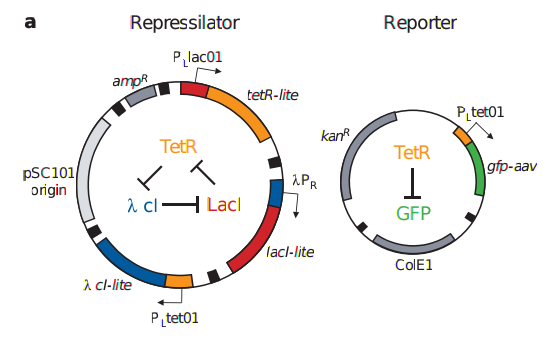
\includegraphics[scale=0.5]{repr.png}
   }
   \frame{
      \frametitle{Design}
      \centering
      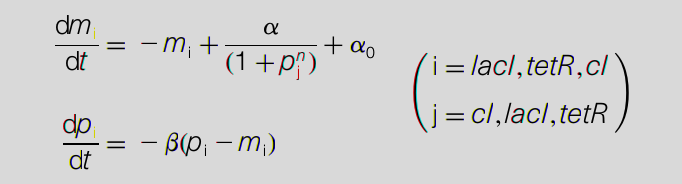
\includegraphics[scale=0.5]{repr_eq.png}
   }

\section{}
   \frame{
      \frametitle{Results}
      \centering
      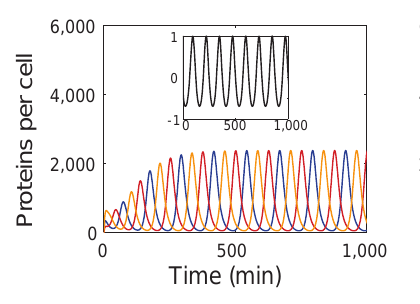
\includegraphics[width=.5\textwidth]{repr_osc_theirs.png}%
      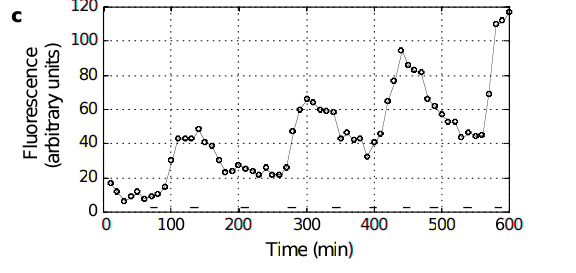
\includegraphics[width=.5\textwidth]{repr_ecoli.png}  
   }
   \frame{
      \frametitle{Results}
      \centering
      \begin{itemize}
         \item Stable oscillations
      \end{itemize} 
      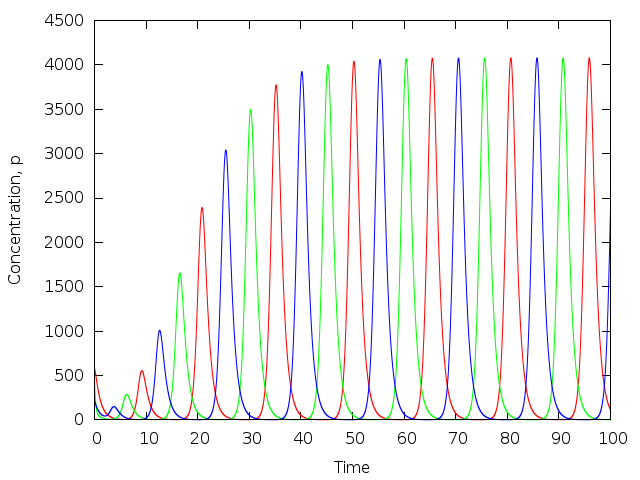
\includegraphics[scale=0.4]{repr_osc.png}
   }
   \frame{
      \frametitle{Results}
      \centering
      \begin{itemize}
         \item Repressor-expressor convergence towards cyclic state
      \end{itemize} 
      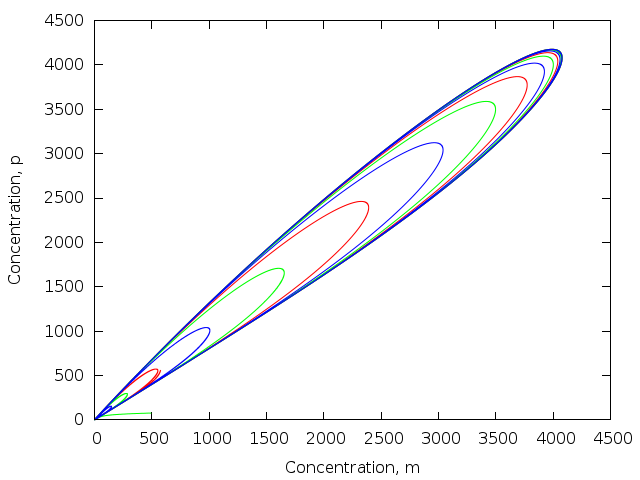
\includegraphics[scale=0.4]{repr_osc_pm.png}
   }
   \frame{
      \frametitle{Results}
      \centering
      \begin{itemize}
         \item Non-oscillating convergence
      \end{itemize} 
      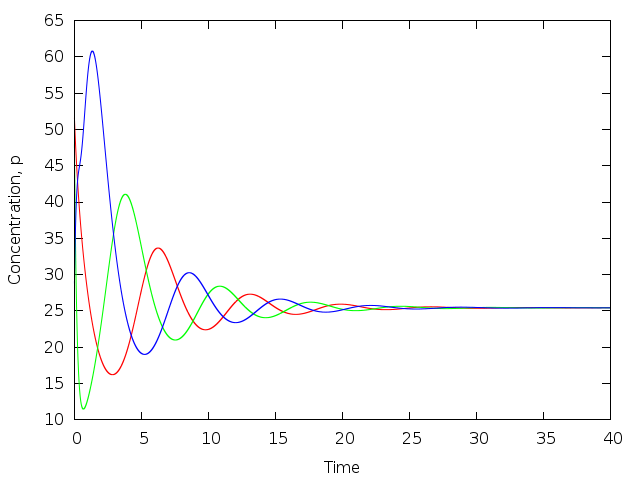
\includegraphics[scale=0.4]{repr_leak.png}
   }
   \frame{
      \frametitle{Results}
      \centering
      \begin{itemize}
         \item Repressor-expressor convergence towards "flat" state.
      \end{itemize} 
      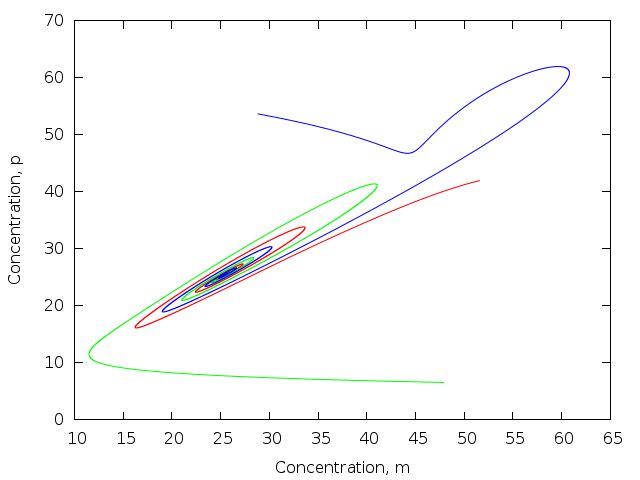
\includegraphics[scale=0.4]{repr_leak_pm.png}
   }

\section{}
   \frame{
      \frametitle{Code}
      \centering
      \begin{itemize}
         \item Implemented in Java
         \item Fourth order Runge-Kutta

      \end{itemize} 
   }


\end{document}

